% THIS IS AN EXAMPLE DOCUMENT FOR VLDB 2012
% based on ACM SIGPROC-SP.TEX VERSION 2.7
% Modified by  Gerald Weber <gerald@cs.auckland.ac.nz>
% Removed the requirement to include *bbl file in here. (AhmetSacan, Sep2012)
% Fixed the equation on page 3 to prevent line overflow. (AhmetSacan, Sep2012)

\documentclass{vldb}
\usepackage{graphicx}
\usepackage{balance}  % for  \balance command ON LAST PAGE  (only there!)


% Include information below and uncomment for camera ready
\vldbTitle{Deferred secondary index update with LSM-trees}
\vldbAuthors{Vladislav Shpilevoy, Konstantin Osipov, Dmitry Volkanov}
\vldbDOI{https://doi.org/TBD}

\begin{document}

% ****************** TITLE ****************************************

\title{Deferred secondary index update with {\ttlit LSM-trees}}

% possible, but not really needed or used for PVLDB:
%\subtitle{[Extended Abstract]
%\titlenote{A full version of this paper is available as\textit{Author's Guide to Preparing ACM SIG Proceedings Using \LaTeX$2_\epsilon$\ and BibTeX} at \texttt{www.acm.org/eaddress.htm}}}

% ****************** AUTHORS **************************************

% You need the command \numberofauthors to handle the 'placement
% and alignment' of the authors beneath the title.
%
% For aesthetic reasons, we recommend 'three authors at a time'
% i.e. three 'name/affiliation blocks' be placed beneath the title.
%
% NOTE: You are NOT restricted in how many 'rows' of
% "name/affiliations" may appear. We just ask that you restrict
% the number of 'columns' to three.
%
% Because of the available 'opening page real-estate'
% we ask you to refrain from putting more than six authors
% (two rows with three columns) beneath the article title.
% More than six makes the first-page appear very cluttered indeed.
%
% Use the \alignauthor commands to handle the names
% and affiliations for an 'aesthetic maximum' of six authors.
% Add names, affiliations, addresses for
% the seventh etc. author(s) as the argument for the
% \additionalauthors command.
% These 'additional authors' will be output/set for you
% without further effort on your part as the last section in
% the body of your article BEFORE References or any Appendices.

\numberofauthors{3} %  in this sample file, there are a *total*
% of EIGHT authors. SIX appear on the 'first-page' (for formatting
% reasons) and the remaining two appear in the \additionalauthors section.

\author{
% You can go ahead and credit any number of authors here,
% e.g. one 'row of three' or two rows (consisting of one row of three
% and a second row of one, two or three).
%
% The command \alignauthor (no curly braces needed) should
% precede each author name, affiliation/snail-mail address and
% e-mail address. Additionally, tag each line of
% affiliation/address with \affaddr, and tag the
% e-mail address with \email.
%
% 1st. author
\alignauthor
Vladislav Shpilevoy
       \affaddr{Lomonosov Moscow State University}\\
       \email{v.shpilevoy@tarantool.org}
% 2nd. author
\alignauthor
Konstantin Osipov
       \affaddr{Tarantool}\\
       \email{kostja@tarantool.org}
% 3rd. author
\alignauthor
Dmitry Volkanov
       \affaddr{Lomonosov Moscow State University}\\
       \email{volkanov@lvk.cs.msu.su}
}
\date{24 January 2018}
% Just remember to make sure that the TOTAL number of authors
% is the number that will appear on the first page PLUS the
% number that will appear in the \additionalauthors section.

\maketitle

\begin{abstract}
Log-Structured merge-trees (LSM-trees) are becoming more and more widely
adopted as a staple data structure in secondary storage database management
systems, ending the half-a-century-long dominance of B-trees. The major
LSM-tree's advantage is that it writes new data and old data updates on disk
always sequentially. It is possible due to LSM-tree's ability to store many
versions of the same key - it allows to LSM-based tables do not read and delete
old data explicitly from primary index on such operations as deletion or replace
to delete old data. Data is deleted by new data during compaction instead. But
this advantage is nullifed by secondary indexes, because replace/delete-like
operations require read and delete old data from each secondary index explicitly.
This paper presents a modification for LSM-tree data structure, which allows to
do not read any index on replace/delete operations even if there are
non-secondary indexes in the table.
Experimental research of the modified LSM-tree shows write speed growth 1.5 to
10 times againts original LSM-tree on tables with 2-4 non-unique secondary
indexes. And the more secondary indexes there are, the faster the new LSM-tree
works on write operations.
\end{abstract}

% Abstract

% -- 1. Introduction
% Краткая история появления LSM-деревьев, предпосылки к этому. Связь с SSD.
% Примеры БД. Главные преимущества (версионность, последовательность записи).
% Главный недостаток - скрытые чтения (что это). На чем проявляются
% (на обновлениях вторичных индексов), на чем нет (только на первичном), почему
% такие плохие. Сказать, что в данной статье представлен алгоритм, который
% позволяет не делать скрытых чтений на некоторых операциях по некоторым таблицам.
% В одно предложение сказать, какой прирост производительности удалось получить.

% -- 2. Background and motivation
% Более полное определение LSM-дерева. Сказать не чрезмерно подробно, какие в нем
% ключевые алгоритмы (как пишутся обновления, как делаются чтения). Сказать про
% ratio размеров уровней.
% -- 2.1. Compaction
% Сказать подробно, как делается слияние уровней, если они представлены
% сортированными массивами (вместо классического варианта, где на диске уровни -
% это B-деревья). Особо упомянуть, что старые данные дискардятся новыми только в
% пределах одинаковых ключей.
% -- 2.2. LSM-tree based index structure
% Про то, что в LSM-tree based таблицах каждый индекс - это LSM-дерево. Первичный
% индекс хранит таплы целиком, вторичный не целиком (это просто упомянуть, так как
% будть индексы хоть covering - это не помогает избавиться от скрытых чтений). Но
% важно, что вторичный индекс использует первичные ключи как ссылки на таплы в
% первичном индексе. И LSM-деревья получаются связанными.
% -- 2.3. Multiple indexes update problem
% Рассказать, что существуют delete и replace операции, которые на одном индексе
% не требуют чтений. Но при появлении вторичных индексов они делают скрытые чтения
% из первичного индекса. В случае replace вторичный ключ может поменяться, и тогда
% во вторичном индексе новая запись не удалит старую. В случае delete по
% первичному ключу есть только первичный ключ, и во вторичные индексы вставлять
% нечего - приходится тоже читать.

% -- 3. Algorithm design and implementation
% Рассказать ключевую идею алгоритма, что скрытые чтения нужны только для удаления
% старых данных, и вместо чтений сразу перед обновлением таблицы можно отложить
% эти чтения до компакта первичного индекса, когда таплы и так и эдак читаются, и
% можно сразу определить, какие таплы дискардятся. Эти таплы можно раскидывать по
% вторичным индексам как delete по вторичным ключам и версиям.
% -- 3.1 Update
% Сказать, что на апдейты более не читаем. Replace пишем сразу во все индексы.
% Delete пишем только в первичный индекс.
% -- 3.2 Compaction
% При компакте первичного индекса собираются таплы, которые собираются удалиться.
% Из них извлекаются вторичные ключи по всем вторичным индексам. Эти ключи вместе
% с версией тапла вставляются в виде delete сразу в дисковую часть каждого
% вторичного индекса. Когда вторичный индекс компактит, он учитывает эти delete,
% причем со сверкой версии - это необходимо, так как delete старых таплов попадают
% по времени во вторичный индекс позже, чем более новые данные.
% -- 3.3 Read
% Читаем как обычно. Все чтения лукапят в первичный индекс. Если там тапл не
% найден, то он пропускается и вторичный индекс читается дальше в соответствии с
% тем, какой был запрос пользователя.
% -- 3.4 Implementaion
% Реализация выполнена на основе БД Tarantool и ее движка Vinyl, который хранит
% данные в LSM-деревьях по ренжам. Ядро нового алгоритма сосредоточено в
% процедуре компакта уровней, где из старых таплов извлекаются вторичные ключи и
% версии, и вставляются сразу на первый уровень (считая с нуля) LSM-деревьев
% вторичных индексов. Пересортировка удаляемых данных первичного индекса в
% порядок вторичных индексов выполняется в памяти по мере чтения схлопываемых
% уровней первичного индекса.

% -- 4. Mathematical basics
% Привести формулы в двух группах: ДО патча и ПОСЛЕ. В каждой группе вывести
% сложность replace, delete, primary get. Учесть level_size_ratio, "ветвистость"
% деревьев в памяти, кол-во таплов в памяти, кол-во уровней на диске и размер
% первого уровня (считая с нуля) первичного индекса.

% -- 5. Evaluation
% Сказать, что наибольший прирост получается при replace/delte операциях и
% зависит, согласно формулам выше, от размеров индексов, ratio и прочего. И что
% кроме наилучшего случая рассмотрен Linkbench. (Постараться сделать сравнения
% не только Тарантула с собой, но и с LevelDB и с MySQL (MyRocks)).
% -- 5.1. Microbench
% Тут показать волшебный прирост 10х, сказать на чем. И сделать такой же тест для
% MyRocks и LevelDB (они усосут, но надо понять, насколько - может еще больше).
% -- 5.2. Linkbench
% Тут показать результаты, которых пока нет, против тех же БД. Ожидается, что
% прирост будет не сказать, что сильно велик, так как там много чтений (явных).

% -- 6. Related work
% Рассказать, что кроме нового алгоритма есть еще куча старых, даже для
% B-деревьев. Чуть-чуть про них рассказать.
% -- 7. Conclusion
% Сказать, что новый алгоритм воскрешает версионность LSM-таблиц со множеством
% индексов. И что можно оптимизировать. Например, при дампе вторичных индексов
% лукапить первичный, чтобы проверять, что какие-то таплы уже может можно и не
% дампить. И помечать такие таплы на диске в первичном индексе, чтобы они при
% удалении во время компакта не создавали делитов.
% И что можно сократить расход памяти во время пересортировки до константного,
% если сделать сортировку слияниями кучки файликов, которые будут копиться во
% время компакта.
% -- 8. References


\section{Introduction}
Log-Structured Merge trees were developed for write-intensive tasks in 1990th
and were used in file systems and for reserve copying. But their prevalence was
restricted by hidden reads.

These are the reads which accompany writes: e.g. when it’s necessary to delete
old data from a secondary index after an update, or check an unique or a foreign
key constraint. A significant amount of reads in a modern database is hidden.
Such reads, when followed by a write, cost nearly nothing in a B-tree, but can
penalize performance of an LSM-tree based table to an extent when its write
advantage becomes completely diluted.

With Solid-State Drive (SSD) appearance cost of random writes had started
contribute to overall performance way more heavily than cost of random reads,
and nowadays the LSM-tree is consideted to be a standard data structure for
databases. For example, it is used in LevelDB, RocksDB, Cassandra, Tarantool,
BigTable, Hbase, Riak, MySQL (MyRocks).

However SSD does not help in a special case, which is very popular and dilutes
LSM-tree's ability to store multiple versions of the same keys. It is linked
with LSM-tree compaction algorithm, and appears on tables with multiple indexes.

In a primary LSM-tree based index any replace or delete operation is executed
with no hidden reads because of LSM-tree ability to store multiple key versions.
A new tuple is just inserted into memory and after some compactions discards old
tuples. But it is not possible if there are secondary indexes. If a table
contains secondary indexes, any update operation must read an old tuple from a
primary index, extract from it secondary keys and delete them from each
secondary index explictly. That is any update of such table produces hidden
reads from a primary index.

Primary index read and explicit old tuple deletion can not be avoided in classic
LSM-tree, because it deletes old versions of the key only if these versions are
equal by the key. If a request changes a secondary key in an exising tuple and
does not deletes old one, then it is not deleted from a secondary index.
LSM-tree considers new and old tuple not to be different versions of the same
key, but to be different keys.

The paper describes a new LSM-tree compaction algorithm, a new LSM-tree based
table update and read algorithms. Replace and delete operations on the new
LSM-tree do not any reads regardless of secondary index number, if all of them
are not unique. Experiments show exponential requests number per second (RPS)
grow on some loading types and some schemas. For example, on a table with 3
non-unique secondary indexes and replace/delete batched requests RPS increased
up to 10 times.

\section{Background and motivation}
This section defines some LSM-tree basics: how it is can be stored on disk and
in memory, how compaction, update and read works. What LSM-tree parameters are
typically configurable.

LSM-tree is a data structure optimized for write-intensive tasks. It has
multiple levels: zero-level is stored in a memory and other on a disk.
Zero-level amasses updates and periodically is dumped on to a disk to become
first level. Zero-level after dump are cleaned up and collects new updates. And
so on.

Zero-level usage allows to write updates to a disk in batches regardless of
their order, keys, types. Even delete is put in a zero-level as a tuple of a
special type.

When level number became too big, the LSM-tree is compacted - several levels are
merged in a new one. During compaction new tuples discard old tuples of the same
key. For example, delete discards all older data and sometimes itself; replace
discards all older data, but not itself.

LSM-tree can store levels in multiple ways. For example, memory level can be
B-tree or Red-Black tree. Disk levels can be organized as B-trees or sorted
arrays. In the paper sorted arrays on disk and B+ tree in memory are considered.

\subsection{Compaction}
\begin{figure}
\centering
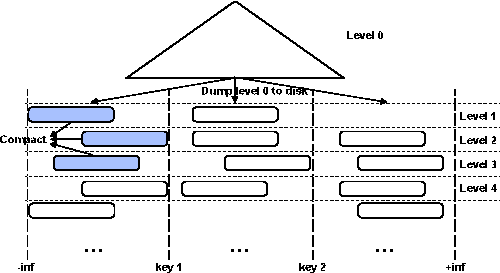
\includegraphics[width=0.4\textwidth]{compaction_schema}
\caption{LSM-tree ranges dump and compaction}
\label{fig:compaction_schema}
\end{figure}
Each level consists of multiple sublevels. Each sublevel is an array sorted by
a key (in a case of LSM-tree index the key consists of index parts) and
containig a specific key values range. During compaction some sublevels of each
levels are merge-sorted into a new sorted array. It is known, that if one key
version is on level $i$ and another on $j < i$, then the key version on level
$j$ is newer and another one is discarded when compacted.

Compaction procecure is needed to reduce level count and to discard old tuples
to make room for new ones. Compaction frequency is regulated by LSM-tree
parameters level size ratio and maximal sublevels count. In each pair of
neighbour levels $i$ and $i + 1$ size of a level $i + 1$ must be greater than
level $i$ size $*$ level size ratio at least. If maximal sublevels count per
level is exceeded or level size ratio is violated, then compaction procedure
merges as much sublevels as needed to satisfy both limitations.

In practice, sublevels are produced by memory level dump and by spliting index
key values into ranges, when each range stores and maintains its own sublevels
independently of other ranges (see Figure \ref{fig:compaction_schema}).

\subsection{LSM-tree based table structure}
In LSM-tree based table each index is an LSM-tree, sorted by the index parts.
It is common pattern, that a table has one primary index and a number of
secondary indexes. A primary index always is unique, and stores full tuples,
including all indexed and not indexed fields, as they were inserted by an user.
A secondary index stores only its own key parts and primary index parts to save
memory. Such indexes are called non-covering. Primary parts are used as link to
a full tuple in a primary index, when a search uses a secondary index only.

The described pattern is not unique feature of LSM-tree based tables. For
example, SQLite secondary indexes based on B-tree are not covering by default
too. And each SQLite table has unique primary index even if an user did not
specified it explicitly.

Since secondary indexes stores primary index parts, they are linked with primary
indexes. And if a tuple does not exist in a primary index, the same tuple can
not exist in a secondary index. This is the reason, why hidden reads are
indispensible - if a tuple is replaced with another secondary key or deleted
from a primary index, then its old version must be deleted from each secondary
index by old secondary key, else a table indexes are not consistent.

\subsection{Multiple indexes update problem}
LSM-tree ability to manage multiple versions of a key allows to avoid hidden
reads on such operations as replace or delete which can not break consistency if
there is only a primary index in a table and no foreign key constraints.
Such operations are known as \textbf{blind-writes} \cite{kai:slimdb}.
Blind-writes are much faster than non-blind insert or update operations, which
read an old tuple in a worst case from a disk to check for duplicate or apply
update operations.

The big problem of LSM-tree based tables is that in presense of secondary
indexes all writes become non-blind. See Figure \ref{fig:inconsistent_example}
for example of inconsistency if replace is blind and a table has secondary
index. Here a table is defined with 4 columns: first is part of a primary index,
2 and 3 are parts of a secondary index, and 4 is not indexed.
\textit{Replace\{1, 5, 6, 7\}} before executed must read old tuple from a
primary index by the key \textit{\{1\}}, extract the secondary key
\textit{\{2, 3\}}, delete it from the secondary index, and only then insert the
new tuple. If the old tuple is not deleted, then during compaction it becames
garbage with no link to a full tuple in the primary index.
\begin{figure}
\centering
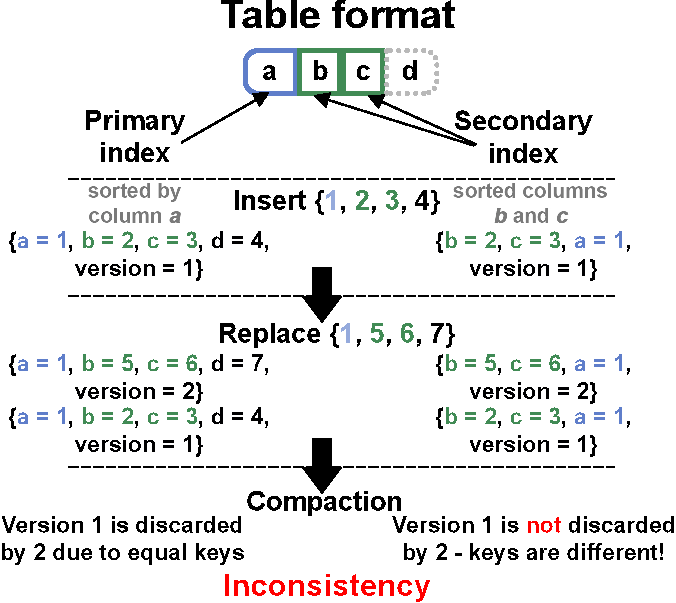
\includegraphics[width=0.3\textwidth]{inconsistent_example}
\caption{LSM-tree based table inconsistency example}
\label{fig:inconsistent_example}
\end{figure}

Since disk access is much slower than memory access, secondary index presence
destroys LSM-tree versions advantage. In the next section a new LSM-tree update
algorithm is presented reviving versions and blind-writes.

\section{Design and implementation}
Below the basics of a new algorithm are described, followed by three sections,
each of which unfolds one of enclosed part of the algorithm.

The key idea of the algorithm is that deletion of old data can be deferred until
primary index compaction stage. It allows to do not hidden reads during replace
and delete by primary key operations since they use hidden reads only to learn
and delete old secondary key versions, not to check consistency. It works on
tables with non-unique secondary indexes only, because it is impossible to break
consistency of non-unique secondary index using delete or replace operations.

Obviously, it is not true if there are unique secondary index. For example,
consider a table with columns \textit{\{a, b\}}, unique primary index on
\textit{\{a\}} and unique secondary index on \textit{\{b\}}. A table contains
two records: \textit{\{1, 1\}} and \textit{\{2, 2\}}. It is impossible now to do
replace \textit{\{1, 2\}}, because it leads to duplicate in the secondary index.

Of course, in MySQL, for example, replace would delete both old records, but
such kind of replace can not be deferred because during the primary index
compaction there is no way to learn that a new tuple with one primary key
discards an old tuple with another primary key without explicitly inserted
deletion. This multi-replace must delete old records with another primary keys,
and it is not considered under the paper.

The algorithm of deferred update consists of three parts:
\begin{enumerate}
\item Update of a zero-level of all indexes. This is where replace and delete by
a primary key are inserted into memory and makes secondary and primary indexes
mal-sinchronized.
\item Compaction, which differs in primary and secondary indexes. A primary
index during compaction detects tuples to discard and sends them to a secondary
indexes as a new LSM-tree sublevel. A secondary index on compaction takes into
account sublevels received from a primary index.
\item Secondary index reading, that now can see tuples already deleted from a
primary index. Existance of a concrete version of a key read from a secondary
index must be check via primary index lookup.
\end{enumerate}

\subsection{Deferred update}

Only two operations can be deferred: replace and delete by a primary key. At
first algorithm of replace exection is presented, and then the delete's one
which is very similar.

Consider a table with one primary index and some non-unique secondary indexes.
Assume an user executes replace. The tuple specified in the replace is inserted
into each indexe's memory level as is, with no preliminary reading and deletion
of an old tuple from secondary indexes.
\begin{figure}
\centering
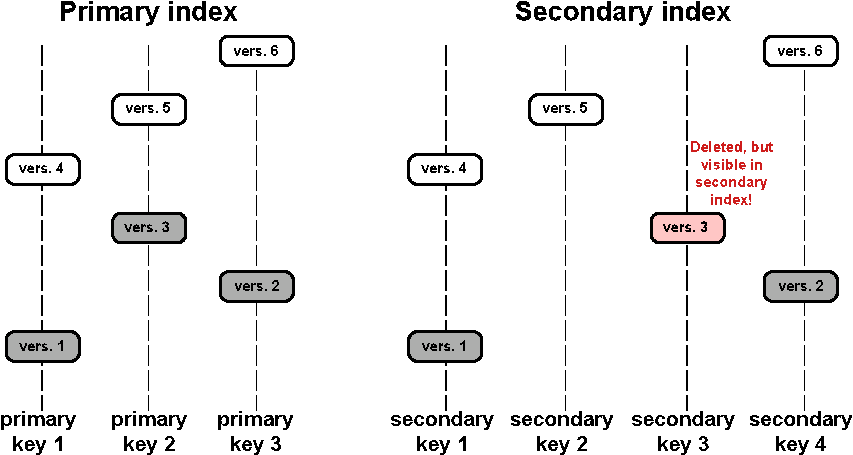
\includegraphics[width=0.46\textwidth]{table_after_deferred_update}
\caption{LSM-tree based table if update is deferred}
\label{fig:table_after_deferred_update}
\end{figure}

When this algorithm is used, it is possible and valid, that some secondary
indexes consider discarded tuples as not discarded, like in example on Figure
\ref{fig:table_after_deferred_update}. In the example there is a tuple with
version 3, which is discarded in a primary index by a newer tuple with the same
key and version 5. But secondary keys of these tuples are different, and a
secondary index sees the tuple with version 3 as a separate non-discarded tuple.

A formula that appears in the running text is called an
inline or in-text formula.  It is produced by the
\textbf{math} environment, which can be
invoked with the usual \texttt{{\char'134}begin. . .{\char'134}end}
construction or with the short form \texttt{\$. . .\$}. You
can use any of the symbols and structures,
from $\alpha$ to $\omega$, available in
\LaTeX\cite{Lamport:LaTeX}; this section will simply show a
few examples of in-text equations in context. Notice how
this equation: \begin{math}\lim_{n\rightarrow \infty}x=0\end{math},
set here in in-line math style, looks slightly different when
set in display style.  (See next section).

\subsubsection{Display Equations}
A numbered display equation -- one set off by vertical space
from the text and centered horizontally -- is produced
by the \textbf{equation} environment. An unnumbered display
equation is produced by the \textbf{displaymath} environment.

Again, in either environment, you can use any of the symbols
and structures available in \LaTeX; this section will just
give a couple of examples of display equations in context.
First, consider the equation, shown as an inline equation above:
\begin{equation}\lim_{n\rightarrow \infty}x=0\end{equation}
Notice how it is formatted somewhat differently in
the \textbf{displaymath}
environment.  Now, we'll enter an unnumbered equation:
\begin{displaymath}\sum_{i=0}^{\infty} x + 1\end{displaymath}
and follow it with another numbered equation:
\begin{equation}\sum_{i=0}^{\infty}x_i=\int_{0}^{\pi+2} f\end{equation}
just to demonstrate \LaTeX's able handling of numbering.

\subsection{Citations}
Citations to articles \cite{bowman:reasoning, clark:pct, braams:babel, herlihy:methodology},
conference
proceedings \cite{clark:pct} or books \cite{salas:calculus, Lamport:LaTeX} listed
in the Bibliography section of your
article will occur throughout the text of your article.
You should use BibTeX to automatically produce this bibliography;
you simply need to insert one of several citation commands with
a key of the item cited in the proper location in
the \texttt{.tex} file \cite{Lamport:LaTeX}.
The key is a short reference you invent to uniquely
identify each work; in this sample document, the key is
the first author's surname and a
word from the title.  This identifying key is included
with each item in the \texttt{.bib} file for your article.

The details of the construction of the \texttt{.bib} file
are beyond the scope of this sample document, but more
information can be found in the \textit{Author's Guide},
and exhaustive details in the \textit{\LaTeX\ User's
Guide}\cite{Lamport:LaTeX}.

This article shows only the plainest form
of the citation command, using \texttt{{\char'134}cite}.
This is what is stipulated in the SIGS style specifications.
No other citation format is endorsed.

\subsection{Tables}
Because tables cannot be split across pages, the best
placement for them is typically the top of the page
nearest their initial cite.  To
ensure this proper ``floating'' placement of tables, use the
environment \textbf{table} to enclose the table's contents and
the table caption.  The contents of the table itself must go
in the \textbf{tabular} environment, to
be aligned properly in rows and columns, with the desired
horizontal and vertical rules.  Again, detailed instructions
on \textbf{tabular} material
is found in the \textit{\LaTeX\ User's Guide}.

Immediately following this sentence is the point at which
Table 1 is included in the input file; compare the
placement of the table here with the table in the printed
dvi output of this document.

\begin{table}
\centering
\caption{Frequency of Special Characters}
\begin{tabular}{|c|c|l|} \hline
Non-English or Math&Frequency&Comments\\ \hline
\O & 1 in 1,000& For Swedish names\\ \hline
$\pi$ & 1 in 5& Common in math\\ \hline
\$ & 4 in 5 & Used in business\\ \hline
$\Psi^2_1$ & 1 in 40,000& Unexplained usage\\
\hline\end{tabular}
\end{table}

To set a wider table, which takes up the whole width of
the page's live area, use the environment
\textbf{table*} to enclose the table's contents and
the table caption.  As with a single-column table, this wide
table will ``float" to a location deemed more desirable.
Immediately following this sentence is the point at which
Table 2 is included in the input file; again, it is
instructive to compare the placement of the
table here with the table in the printed dvi
output of this document.


\begin{table*}
\centering
\caption{Some Typical Commands}
\begin{tabular}{|c|c|l|} \hline
Command&A Number&Comments\\ \hline
\texttt{{\char'134}alignauthor} & 100& Author alignment\\ \hline
\texttt{{\char'134}numberofauthors}& 200& Author enumeration\\ \hline
\texttt{{\char'134}table}& 300 & For tables\\ \hline
\texttt{{\char'134}table*}& 400& For wider tables\\ \hline\end{tabular}
\end{table*}
% end the environment with {table*}, NOTE not {table}!

\subsection{Figures}
Like tables, figures cannot be split across pages; the
best placement for them
is typically the top or the bottom of the page nearest
their initial cite.  To ensure this proper ``floating'' placement
of figures, use the environment
\textbf{figure} to enclose the figure and its caption.

This sample document contains examples of \textbf{.pdf} files to be
displayable with \LaTeX (See Figures \ref{fig:fly} and \ref{fig:bigfly}).  More details on each of these is found in the
\textit{Author's Guide}.

\begin{figure}
\centering

\includegraphics{fly}
\caption{A sample black and white graphic (.pdf format).}
\label{fig:fly}
\end{figure}

\begin{figure}
\centering

\includegraphics[width=1in,height=1in]{fly}
\caption{A sample black and white graphic (.pdf format)
that has been resized with the \texttt{includegraphics} command.}
\label{fig:bigfly}
\end{figure}


As was the case with tables, you may want a figure
that spans two columns.  To do this, and still to
ensure proper ``floating'' placement of tables, use the environment
\textbf{figure*} to enclose the figure and its caption (See Figure~\ref{fig:flies}). And don't forget to end the environment with {figure*}, not {figure}!

\begin{figure*}
\centering
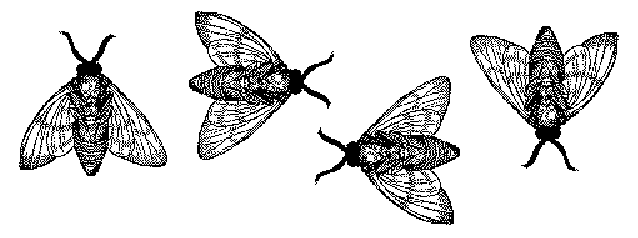
\includegraphics{flies}
\caption{A sample black and white graphic (.pdf format)
that needs to span two columns of text.}
\label{fig:flies}
\end{figure*}


Note that only {\textbf{.pdf}} files were used; if you want to include
{\textbf{.ps}} or {\textbf{.eps}} formats, you can use the
\texttt{{\char'134}epsfig} or \texttt{{\char'134}psfig}
commands as appropriate for the different file types.

\subsection{Theorem-like Constructs}
Other common constructs that may occur in your article are
the forms for logical constructs like theorems, axioms,
corollaries and proofs.  There are
two forms, one produced by the
command \texttt{{\char'134}newtheorem} and the
other by the command \texttt{{\char'134}newdef}; perhaps
the clearest and easiest way to distinguish them is
to compare the two in the output of this sample document:

This uses the \textbf{theorem} environment, created by
the\linebreak\texttt{{\char'134}newtheorem} command:
\newtheorem{theorem}{Theorem}
\begin{theorem}
Let $f$ be continuous on $[a,b]$.  If $G$ is
an antiderivative for $f$ on $[a,b]$, then
\begin{displaymath}\int^b_af(t)dt = G(b) - G(a).\end{displaymath}
\end{theorem}

The other uses the \textbf{definition} environment, created
by the \texttt{{\char'134}newdef} command:
\newdef{definition}{Definition}
\begin{definition}
If $z$ is irrational, then by $e^z$ we mean the
unique number which has
logarithm $z$: \begin{displaymath}{\log e^z = z}\end{displaymath}
\end{definition}

Two lists of constructs that use one of these
forms is given in the
\textit{Author's  Guidelines}.


There is one other similar construct environment, which is
already set up
for you; i.e. you must \textit{not} use
a \texttt{{\char'134}newdef} command to
create it: the \textbf{proof} environment.  Here
is a example of its use:
\begin{proof}
Suppose on the contrary there exists a real number $L$ such that
\begin{displaymath}
\lim_{x\rightarrow\infty} \frac{f(x)}{g(x)} = L.
\end{displaymath}
Then
\begin{align*}
l&=\lim_{x\rightarrow c} f(x)
= \lim_{x\rightarrow c}
\left[ g{x} \cdot \frac{f(x)}{g(x)} \right ] \\
&= \lim_{x\rightarrow c} g(x) \cdot \lim_{x\rightarrow c}
\frac{f(x)}{g(x)} = 0\cdot L = 0,
\end{align*}
which contradicts our assumption that $l\neq 0$.
\end{proof}

Complete rules about using these environments and using the
two different creation commands are in the
\textit{Author's Guide}; please consult it for more
detailed instructions.  If you need to use another construct,
not listed therein, which you want to have the same
formatting as the Theorem
or the Definition\cite{salas:calculus} shown above,
use the \texttt{{\char'134}newtheorem} or the
\texttt{{\char'134}newdef} command,
respectively, to create it.

\subsection*{A {\secit Caveat} for the \TeX\ Expert}
Because you have just been given permission to
use the \texttt{{\char'134}newdef} command to create a
new form, you might think you can
use \TeX's \texttt{{\char'134}def} to create a
new command: \textit{Please refrain from doing this!}
Remember that your \LaTeX\ source code is primarily intended
to create camera-ready copy, but may be converted
to other forms -- e.g. HTML. If you inadvertently omit
some or all of the \texttt{{\char'134}def}s recompilation will
be, to say the least, problematic.

\section{Conclusions}
This paragraph will end the body of this sample document.
Remember that you might still have Acknowledgments or
Appendices; brief samples of these
follow.  There is still the Bibliography to deal with; and
we will make a disclaimer about that here: with the exception
of the reference to the \LaTeX\ book, the citations in
this paper are to articles which have nothing to
do with the present subject and are used as
examples only.
%\end{document}  % This is where a 'short' article might terminate

% ensure same length columns on last page (might need two sub-sequent latex runs)
\balance

%ACKNOWLEDGMENTS are optional
\section{Acknowledgments}
This section is optional; it is a location for you
to acknowledge grants, funding, editing assistance and
what have you.  In the present case, for example, the
authors would like to thank Gerald Murray of ACM for
his help in codifying this \textit{Author's Guide}
and the \textbf{.cls} and \textbf{.tex} files that it describes.


% The following two commands are all you need in the
% initial runs of your .tex file to
% produce the bibliography for the citations in your paper.
\bibliographystyle{abbrv}
\bibliography{vldb_sample}  % vldb_sample.bib is the name of the Bibliography in this case
% You must have a proper ".bib" file
%  and remember to run:
% latex bibtex latex latex
% to resolve all references

\subsection{References}
Generated by bibtex from your ~.bib file.  Run latex,
then bibtex, then latex twice (to resolve references).

%APPENDIX is optional.
% ****************** APPENDIX **************************************
% Example of an appendix; typically would start on a new page
%pagebreak

\begin{appendix}
You can use an appendix for optional proofs or details of your evaluation which are not absolutely necessary to the core understanding of your paper. 

\section{Final Thoughts on Good Layout}
Please use readable font sizes in the figures and graphs. Avoid tempering with the correct border values, and the spacing (and format) of both text and captions of the PVLDB format (e.g. captions are bold).

At the end, please check for an overall pleasant layout, e.g. by ensuring a readable and logical positioning of any floating figures and tables. Please also check for any line overflows, which are only allowed in extraordinary circumstances (such as wide formulas or URLs where a line wrap would be counterintuitive).

Use the \texttt{balance} package together with a \texttt{\char'134 balance} command at the end of your document to ensure that the last page has balanced (i.e. same length) columns.

\end{appendix}



\end{document}
